\documentclass[conference]{IEEEtran}
\usepackage[T1]{fontenc}
\usepackage[utf8]{inputenc}
\usepackage[brazil]{babel}
\usepackage{amsmath,amssymb,graphicx,booktabs,url}
\usepackage{balance}
\usepackage[hidelinks]{hyperref}
\graphicspath{{imagens/}}
\title{AERIS: Gaussian Splatting e Composição Multicamada em uma Estação de Monitoramento Aéreo}
\author{\IEEEauthorblockN{Matheus Della Rosa e Guilherme Marolla Tesch}
\IEEEauthorblockA{Engenharia de Computação --- Computação Gráfica e Visualização Científica\\
RA 113209 \qquad RA 113800}}
\begin{document}
\maketitle
\begin{abstract}
Apresenta-se uma estação interativa de monitoramento aéreo para uma missão sintética de reconhecimento de incêndios. A aplicação combina terreno tridimensional representado por Gaussianas anisotrópicas, fumaça, focos de calor, navegação e instrumentos em OpenGL 3.3. Implementam-se projeção perspectiva de covariâncias, descarte de primitivas invisíveis, ordenação por profundidade e rasterização por quads instanciados. Um cache separa componentes estáticos e dinâmicos. As estratégias monolítica e multicamada recebem os mesmos dados e preservam a ordem de desenho. A avaliação utiliza quatro cargas, duas resoluções e três repetições. Na plataforma AMD Vega 8, a latência média multicamada superou a monolítica em todas as configurações avaliadas. Amostras brutas e metadados permitem auditar a análise. Os resultados descrevem o ambiente medido, sem estabelecer garantias temporais.
\end{abstract}
\begin{IEEEkeywords}
Gaussian splatting, composição gráfica, visualização interativa, monitoramento aéreo, desempenho.
\end{IEEEkeywords}

\section{Introdução}
Uma estação de monitoramento reúne informações de natureza distinta: representação do terreno, posição de veículos, estado da missão e alertas. Quando a visualização inclui transparências e sobreposições, a organização do pipeline influencia tanto a qualidade da imagem quanto o custo de cada quadro. Separar funções em camadas facilita inspeção, mas acrescenta texturas, mudanças de destino e passes de composição.

O AERIS investiga essa relação em uma missão procedural de inspeção de incêndios na Serra do Mar. O cenário é uma estação terrestre de drone, adaptando a organização por subsistemas de trabalhos de composição aviônica para uma finalidade ambiental. A geometria e a telemetria são sintéticas; o nome geográfico não representa levantamento real. O usuário altera câmera, cenário, carga e visibilidade durante a execução.

A pergunta experimental é: qual é o custo observado da composição em duas ou quatro camadas, em relação ao desenho direto, quando conteúdo, ordem e transparência são equivalentes? A resposta requer controle dos dados e distinção entre medição e interpretação. FPS sozinho pode ocultar dispersão ou atrasos ocasionais.

As contribuições são uma implementação explícita de projeção, ordenação e rasterização de Gaussianas; uma cena interativa com cache de partes estáticas; um pipeline compartilhado que reduz diferenças acidentais entre estratégias; e coleta auditável com repetições e metadados. A separação gráfica não constitui separação de processos ou de recursos temporais.

\section{Trabalhos relacionados}
Barladian et al.~\cite{barladian} estudam composição de múltiplas janelas com OpenGL SC e JetOS. O AERIS utiliza a distinção entre produção das imagens e composição, mas executa em contexto compartilhado num computador convencional. A mudança de plataforma impede transferir os resultados do artigo para esta implementação.

Trompouki e Kosmidis~\cite{trompouki} revisam métodos de certificação de software de aplicação em GPU. A referência situa exigências de verificação além de testes de desempenho. Aqui, percentis e máximos são descrições amostrais, sem análise de pior caso ou processo de certificação.

Kerbl et al.~\cite{kerbl} apresentam representação e renderização por Gaussianas 3D com otimização da cena. Este protótipo implementa splatting procedural, sem reconstrução fotográfica, treinamento, controle adaptativo de densidade ou harmônicos esféricos. Essa delimitação permite estudar o algoritmo gráfico sem acrescentar aprendizado.

\section{Metodologia e modelagem}
\subsection{Arquitetura}
O sistema é organizado em dados, representação, renderização e composição. O simulador fornece snapshots independentes com semente local e passo explícito. A representação constrói painéis e uma carga adicional de retângulos. O renderizador utiliza buffers persistentes para triângulos e atlas de fontes. O compositor administra texturas RGBA8 e framebuffers intermediários.

A cena 3D ocupa um painel delimitado por viewport. Navegação, instrumentos e alertas formam os outros grupos lógicos. Em quatro camadas, cada grupo possui uma textura. Em duas, terreno e navegação são agrupados, assim como instrumentos e alertas. A câmera orbital responde ao arraste e à roda do mouse. Pausa e reinício permitem observar o mesmo estado em diferentes modos.

\begin{figure}[t]
\centering
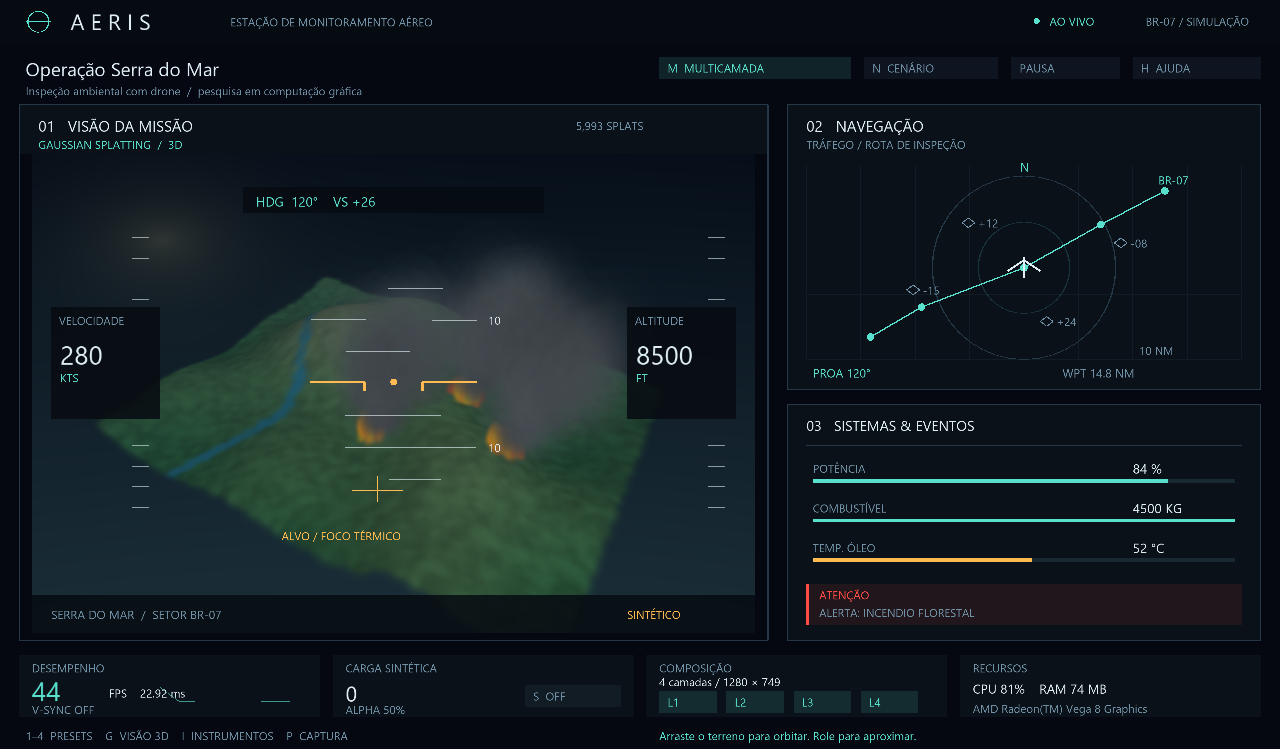
\includegraphics[width=\columnwidth]{aeris.png}
\caption{Estação AERIS com terreno e incêndios sintéticos, navegação, instrumentos e métricas.}
\label{fig:interface}
\end{figure}

\subsection{Representação por Gaussianas}
Cada primitiva possui centro $\boldsymbol{\mu}\in\mathbb{R}^3$, covariância simétrica $\Sigma\in\mathbb{R}^{3\times3}$ e cor RGBA. No terreno, a covariância acompanha a inclinação local do relevo; fumaça e fogo utilizam escalas próprias. A geração emprega semente fixa para reconstruir o conjunto.

Se $R$ e $\mathbf{t}$ transformam mundo em câmera, o centro é $\mathbf{p}=R\boldsymbol{\mu}+\mathbf{t}$. Definindo $d=-p_z>0$, sua projeção normalizada é
\begin{equation}
\boldsymbol{\mu}_{2D}=
\begin{pmatrix} f_xp_x/d \\ f_yp_y/d \end{pmatrix}.
\end{equation}
A Jacobiana é
\begin{equation}
J=\begin{pmatrix}
f_x/d & 0 & f_xp_x/d^2\\
0 & f_y/d & f_yp_y/d^2
\end{pmatrix},
\end{equation}
e a covariância projetada resulta da aproximação local
\begin{equation}
\Sigma_{2D}=J R\Sigma R^{T}J^{T}.
\end{equation}
Autovalores e autovetores definem os eixos da elipse em tela. Um piso subpixel na diagonal evita degeneração de splats pequenos. A GPU recebe apenas centro, dois eixos e cor por instância.

Primitivas fora dos planos near e far, atrás da câmera ou com dados inválidos são descartadas antes da divisão perspectiva. O teste lateral considera o suporte de três desvios padrão da elipse, preservando contribuições que atravessam a borda. Testar apenas o centro causaria desaparecimento prematuro de primitivas grandes.

\subsection{Ordenação e rasterização}
A transparência depende da ordem. Os centros são ordenados do fundo para a frente, com desempate pelo identificador original. Essa escolha mantém a imagem determinística quando duas profundidades coincidem. A ordenação global tem custo geral $O(N\log N)$, sem particionamento por tiles.

Um quad é instanciado para cada Gaussiana visível. O vertex shader transforma seus cantos pelos eixos da elipse. Para a coordenada local $\mathbf{q}$, o fragment shader calcula
\begin{equation}
\alpha(\mathbf{q})=\alpha_0\exp\left(-\tfrac12\|\mathbf{q}\|^2\right).
\end{equation}
Fragmentos além de $3\sigma$ ou com contribuição inferior a $1/255$ são descartados. O suporte finito reduz o trabalho sobre contribuições desprezíveis e explicita uma aproximação do método.

Terreno e centros dos focos permanecem fixos. Sua projeção, descarte e autovetores ficam em cache por câmera e resolução. Apenas a fumaça exige nova projeção durante a animação; a opacidade do fogo varia sem mover seus centros. Os conjuntos são reunidos e reordenados globalmente. Durante a pausa, reutiliza-se também o lote de instâncias. A equivalência com o cálculo integral é verificada numericamente.

\subsection{Composição}
Todos os shaders produzem cor pré-multiplicada $\mathbf{c}_p=\alpha\mathbf{c}$. Para fonte $s$ e destino $d$, a composição usa
\begin{align}
\mathbf{c}_{out}&=\mathbf{c}_{p,s}+(1-\alpha_s)\mathbf{c}_{p,d},\\
\alpha_{out}&=\alpha_s+(1-\alpha_s)\alpha_d.
\end{align}
O mesmo contrato atende primitivas, fontes, Gaussianas e texturas intermediárias. Aplicar alpha novamente à cor já acumulada produziria escurecimento indevido nas bordas.

No modo monolítico, todos os grupos escrevem diretamente no destino final. Existem vários draw calls, porém uma passagem de destino, sem texturas intermediárias. No multicamada, cada grupo escreve em FBO próprio, seguido da composição ordenada. Em ambos, formas e textos de um grupo terminam antes do grupo seguinte. Agrupar globalmente os textos alteraria sua sobreposição e invalidaria a comparação.

A quantização RGBA8 pode produzir pequenas diferenças entre os percursos. Os testes de pixels medem essas diferenças, limitando erro máximo e médio. A visibilidade aplica a mesma máscara nas duas estratégias. O redimensionamento recria anexos e atualiza a escala do texto.

\section{Avaliação experimental}
\subsection{Estruturas e sequência de execução}
A geometria é mantida em arrays contíguos, evitando criar objetos Python por primitiva a cada quadro. As funções numéricas de projeção não dependem do contexto OpenGL, o que permite verificar a modelagem por testes de referência. Dados de entrada são validados antes da projeção. Covariâncias não finitas, profundidades inválidas e primitivas invisíveis não chegam ao lote de instâncias.

O cache não substitui o desenho do terreno por uma imagem estática. Mesmo com câmera fixa, seus splats continuam participando da rasterização e da composição a cada quadro; somente a preparação CPU é reaproveitada. Portanto, a fumaça permanece corretamente integrada na ordem global. Alterar a câmera ou a dimensão do painel reconstrói a projeção estática antes de combinar os conjuntos.

\begin{table}[t]
\centering
\caption{Sequência central por quadro, comum às estratégias.}
\begin{tabular}{lp{6.9cm}}
\toprule
Passo & Operação\\
\midrule
1 & Receber snapshot e definir câmera e viewport.\\
2 & Invalidar cache se câmera ou resolução mudarem.\\
3 & Projetar terreno e focos apenas quando necessário.\\
4 & Atualizar e projetar fumaça; combinar profundidades.\\
5 & Ordenar com desempate por identificador original.\\
6 & Instanciar quads; rasterizar densidade e alpha.\\
7 & Desenhar os instrumentos na ordem funcional.\\
8 & Compor texturas intermediárias no modo multicamada.\\
\bottomrule
\end{tabular}
\end{table}

A memória das instâncias tem custo linear: cada Gaussiana visível ocupa dez floats, ou 40 bytes no lote GPU. Para 6.000 primitivas, esse lote soma aproximadamente 234 KiB, sem incluir os arrays de origem, os índices de ordenação e o cache CPU. Cada retângulo sintético utiliza seis vértices com seis floats; 100.000 retângulos correspondem a aproximadamente 13,73 MiB de dados geométricos. Essas quantidades descrevem estruturas, não o consumo total do processo ou do driver.

Os buffers de primitivas crescem quando a capacidade é excedida, sem descartar silenciosamente vértices. A liberação explícita ocorre enquanto o contexto permanece válido. No redimensionamento, a referência ao framebuffer padrão pode conservar dimensões iniciais na biblioteca; por isso, o aplicativo usa a dimensão real comunicada pela janela, e o benchmark utiliza anexos offscreen de tamanho fixo. Esse detalhe evita confundir uma mudança de tamanho visual com a resolução efetivamente processada.

\subsection{Protocolo}
A matriz mantém a cena de 6.000 Gaussianas e varia retângulos adicionais. C1 a C4 são escolhas deste projeto. A carga é dividida exatamente entre as camadas, inclusive quando a quantidade não é divisível pelo número de grupos.

\begin{table}[t]
\centering
\caption{Matriz de avaliação de composição.}
\begin{tabular}{lrrl}
\toprule
Config. & Retângulos & Camadas & Resolução\\
\midrule
C1 & 1.000 & 2 & $1280\times720$\\
C2 & 10.000 & 2 & $1280\times720$\\
C3 & 50.000 & 4 & $1280\times720$\\
C4 & 100.000 & 4 & $1920\times1080$\\
\bottomrule
\end{tabular}
\end{table}

Utiliza-se cenário de incêndio, semente 42 e 50\% dos retângulos com alpha inferior a um. Descartam-se 60 quadros de aquecimento por execução. Medem-se 180 quadros em cada uma das três repetições. A ordem das estratégias alterna entre repetições e configurações. Cada par recebe a mesma sequência pré-calculada, com passo de $1/60$ s. Isso remove a dependência entre estado simulado e velocidade do renderizador.

Ambos os modos usam destino offscreen RGBA8 na resolução exata do preset, sem MSAA. O limite físico da janela e a escala de DPI não alteram a resolução efetiva. V-Sync e apresentação não participam da coleta. Cada duração inclui preparação da geometria, comandos, rasterização, composição e espera por conclusão com \texttt{finish}. A medida é latência conjunta CPU e GPU sincronizada.

Exportam-se tempo por frame, média, desvio padrão, mediana, P95, P99, máximo observado e frequência acima de 16,67 ms. FPS é $1000/\bar{t}$, evitando a média dos inversos individuais. CPU é calculada por segundos de processo divididos pelo tempo de parede. Memória é RSS amostrada; VRAM total do processo não é medida.

\subsection{Resultados}
A coleta ocorreu em 21 de outubro de 2026, no Windows 10, Python 3.14.7 e AMD Radeon Vega 8, com OpenGL 3.3. Foram medidos 4.320 quadros (540 por combinação) após descartar 1.440 de aquecimento. O destino offscreen de C4 manteve $1920\times1080$ pixels, apesar dos limites do monitor.

\begin{table}[t]

\centering

\caption{Resultados agregados de três repetições.}

\label{tab:resultados}

\begin{tabular}{llrrr}

\toprule

Config. & Modo & Média (ms) & P99 (ms) & FPS \\

\midrule

C1 & Mono & 20.83 & 28.38 & 48.01 \\

C1 & Multi & 23.19 & 31.71 & 43.13 \\

C2 & Mono & 21.30 & 30.68 & 46.94 \\

C2 & Multi & 23.81 & 35.09 & 42.00 \\

C3 & Mono & 20.87 & 27.57 & 47.91 \\

C3 & Multi & 24.16 & 27.74 & 41.40 \\

C4 & Mono & 30.76 & 47.63 & 32.51 \\

C4 & Multi & 34.43 & 45.08 & 29.05 \\

\bottomrule

\end{tabular}

\end{table}

A média multicamada foi maior nas quatro configurações: 11.3\%, 11.8\%, 15.7\%, 11.9\%, respectivamente. Esse resultado é compatível com o custo adicional de destinos intermediários e passes de tela cheia. Ele não isola o tempo de cada mecanismo, pois a medida conjunta inclui CPU, rasterização e sincronização.

Em C4, as médias foram 30,76 ms (monolítica) e 34,43 ms (multicamada), correspondendo a 32,51 e 29,05 FPS. O P99 multicamada, 45,08 ms, foi inferior aos 47,63 ms monolíticos nessa coleta. Portanto, média e cauda não devem ser confundidas, nem se pode concluir superioridade temporal geral por uma única métrica.

Todos os quadros medidos ultrapassaram o orçamento de 16,67 ms. A cena desta avaliação não sustentou 60 FPS sincronizados nessa máquina. A fluidez interativa observada em outras condições não altera esse resultado do experimento.

Os valores de C1 a C3 permaneceram próximos e não cresceram monotonicamente com a carga. O custo da cena 3D, a posição concentrada dos retângulos e a variação do sistema limitam inferências sobre escalabilidade. C4 altera simultaneamente resolução e carga; esse contraste não permite atribuir a diferença exclusivamente a uma delas.

A RSS média variou aproximadamente de 96 a 120 MiB. Essa medida inclui Python e caches do driver no processo compartilhado; não deve ser interpretada como memória exclusiva dos FBOs. Para quatro texturas RGBA8 em 1080p, apenas os anexos de cor intermediários somam cerca de 31,64 MiB, excluindo alvos finais, buffers e overhead do driver.

Os arquivos de amostras, resumos por repetição, capturas e metadados estão preservados na execução \texttt{20261021T030448Z\_7e3fc562}. Gráficos apresentam dispersão e médias; nenhuma diferença foi submetida a teste de significância.
\begin{figure*}[t]
\centering
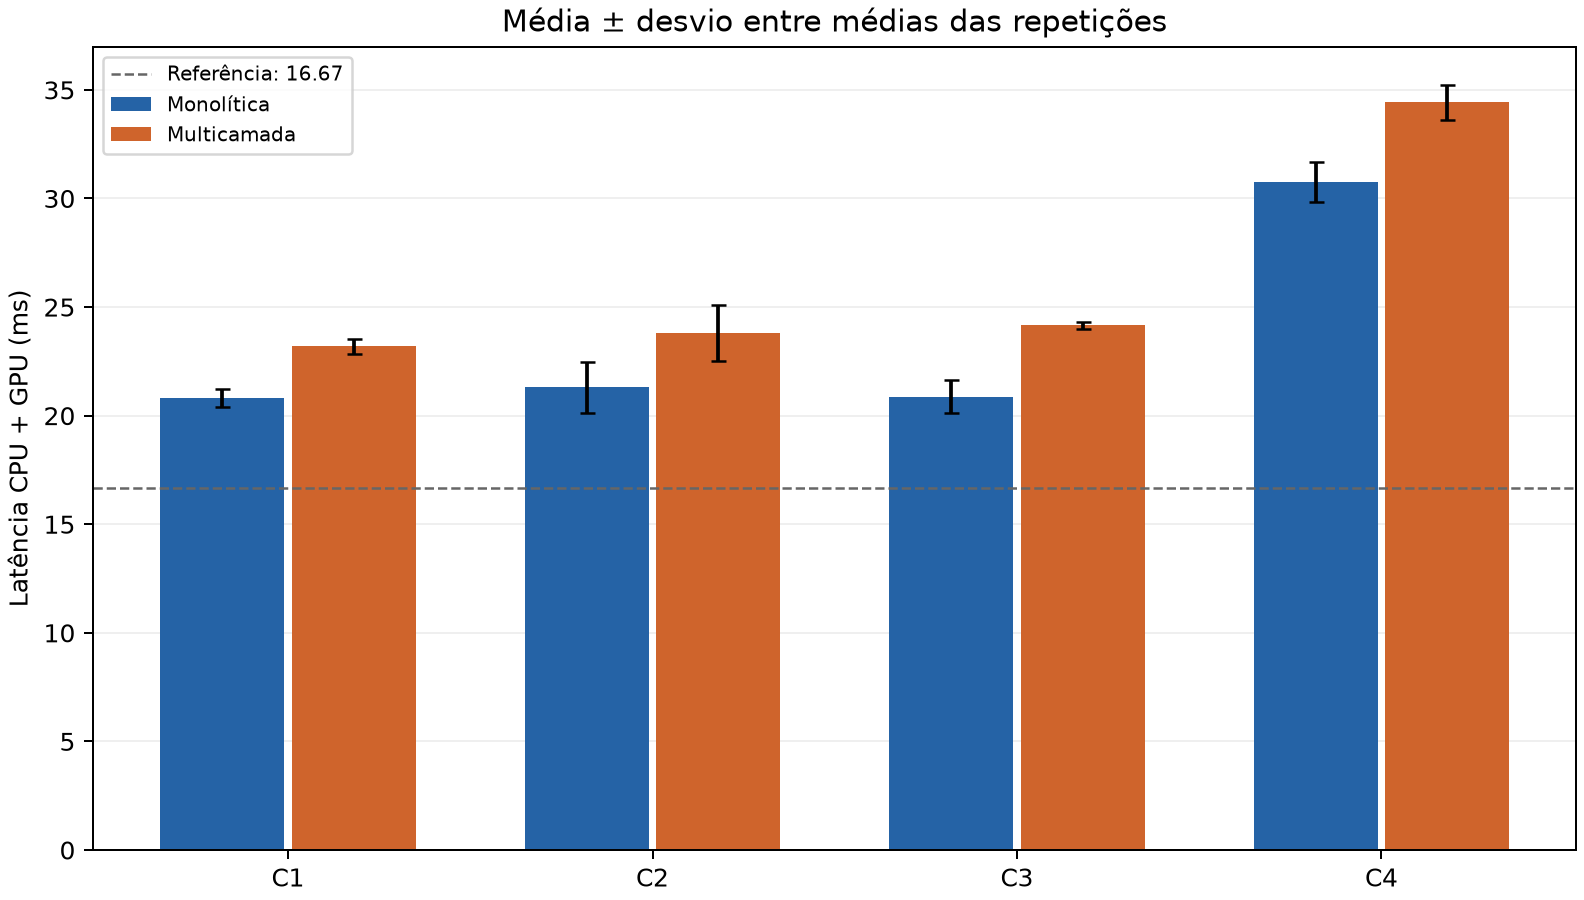
\includegraphics[width=.485\textwidth]{comparativo_tempo_frame.png}
\hfill
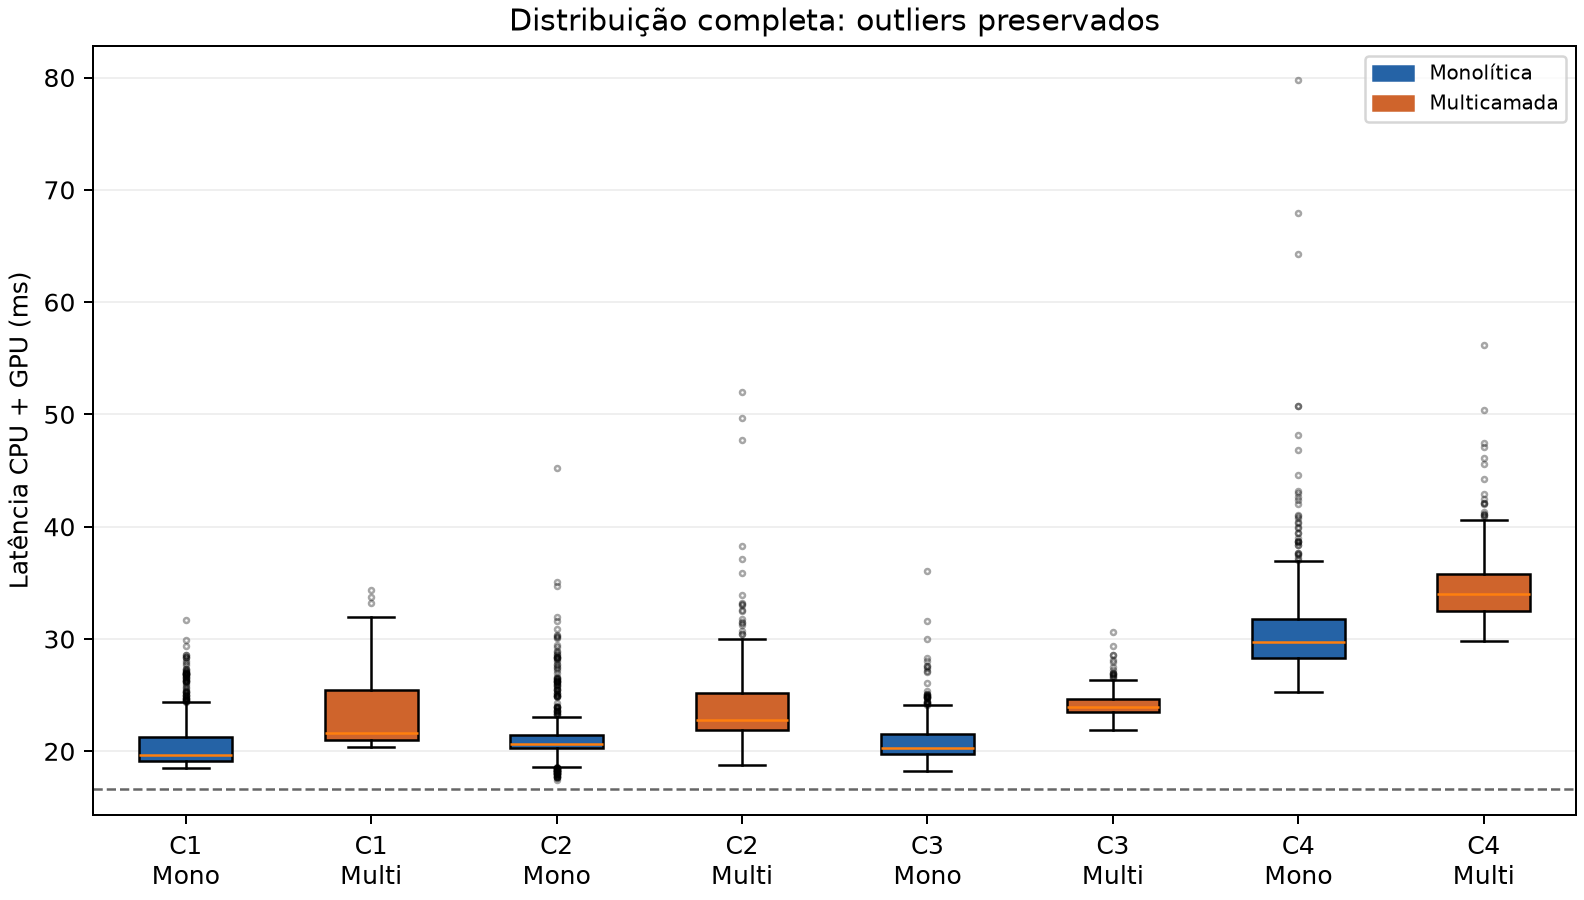
\includegraphics[width=.485\textwidth]{distribuicao_tempo_frame.png}
\caption{Esquerda: latência CPU e GPU; barras de erro representam o desvio padrão entre médias das repetições, sem interpretação como intervalo de confiança. Direita: distribuição completa dos tempos por quadro, com valores extremos preservados.}
\label{fig:latencia}
\end{figure*}

\subsection{Validação}
Os testes numéricos verificam perspectiva, covariância, near/far, suporte no frustum, ordenação estável e entradas inválidas. O cache é comparado ao cálculo integral sob diferentes câmeras, resoluções, instantes e cenários. A simulação verifica determinismo, pausa sem consumo de aleatoriedade e reinício.

\balance
Testes com OpenGL real cobrem alpha, fontes, buffers expansíveis, visibilidade, redimensionamento e liberação idempotente. Comparações da cena completa incluem cenários normal, tráfego e incêndio em duas e quatro camadas. Os pares usam o mesmo estado e leitura RGBA8. A tolerância limita erro máximo, percentil e média para distinguir quantização de falhas de composição.

\subsection{Ameaças à validade}
O experimento ocorre numa sessão de computador convencional. Frequências dinâmicas, atividade de outros processos, temperatura e caches do driver influenciam os tempos. Alternar a ordem reduz um viés, mas não constitui controle completo. As três repetições descrevem esta execução e não sustentam generalização a todas as GPUs.

A ordenação por centro aproxima a visibilidade de Gaussianas que se interpenetram. Não há ordenação exata por fragmento ou rasterização em tiles. A cena procedural também não mede precisão geográfica, detecção de incêndio real ou acurácia de sensores. Os retângulos adicionais estressam composição e sobreposição; não equivalem ao mesmo número de Gaussianas.

Há uma distinção entre independência visual e isolamento computacional. Ocultar um grupo demonstra controle de composição, mas todos os grupos compartilham CPU, contexto e GPU. Não se mediram contenção de falhas ou comportamento sob perda de dados. A amostragem de CPU e RSS ocorre fora da duração individual do quadro, enquanto o tempo total da coleta ainda inclui esse custo de observação. Essa diferença é registrada para tornar comparáveis as definições de cada métrica.

\section{Conclusão e trabalhos futuros}
O AERIS integra uma cena 3D e instrumentos transparentes com duas estratégias de composição comparáveis. O núcleo implementa projeção anisotrópica, descarte, ordenação e rasterização de Gaussianas, com cache para partes estáticas. A coleta preserva amostras e parâmetros, permitindo reexaminar conclusões sem depender de números transcritos.

Os resultados são custos observados na plataforma descrita. A organização multicamada oferece controle funcional, mas não implica menor latência ou melhor previsibilidade. Percentis e máximos amostrais não garantem prazos. O protótipo não implementa escalonamento de tempo real ou isolamento certificado.

Trabalhos futuros incluem consultas de tempo GPU, múltiplas máquinas, câmeras em movimento e variação sistemática do número de Gaussianas. Atualização diferencial de camadas, ordenação por tiles e nível de detalhe podem alterar a relação entre custo e qualidade. Dados geográficos reais exigiriam avaliação de precisão e procedência.

\begin{thebibliography}{3}
\bibitem{barladian}
B. Kh. Barladian et al., \emph{Multi-windows Rendering Using Software OpenGL in Avionics Embedded Systems}, GraphiCon, CEUR Workshop Proceedings, vol. 2485, pp. 28--31, 2019. \url{https://ceur-ws.org/Vol-2485/paper7.pdf}.
\bibitem{trompouki}
M. M. Trompouki and L. Kosmidis, \emph{DO-178C Certification of General-Purpose GPU Software: Review of Existing Methods and Future Directions}, IEEE/AIAA DASC, 2021, pp. 1--9. doi:10.1109/DASC52595.2021.9594412.
\bibitem{kerbl}
B. Kerbl, G. Kopanas, T. Leimkühler, and G. Drettakis, \emph{3D Gaussian Splatting for Real-Time Radiance Field Rendering}, ACM Transactions on Graphics, vol. 42, no. 4, 2023. doi:10.1145/3592433.
\end{thebibliography}
\end{document}
